\section{Hardware \& software realization}
blah \autoref{fig:LSRQuadAndTri}

\begin{figure}[ht]
 \centering
 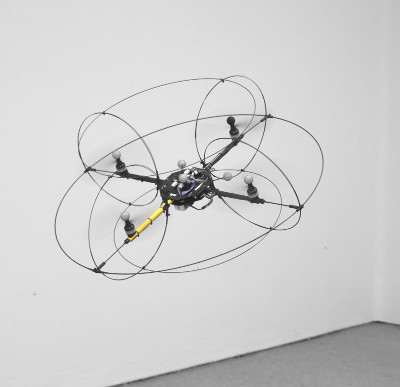
\includegraphics[width=.45\linewidth]{QuadV4.jpg}
 \hspace{.05\linewidth}
 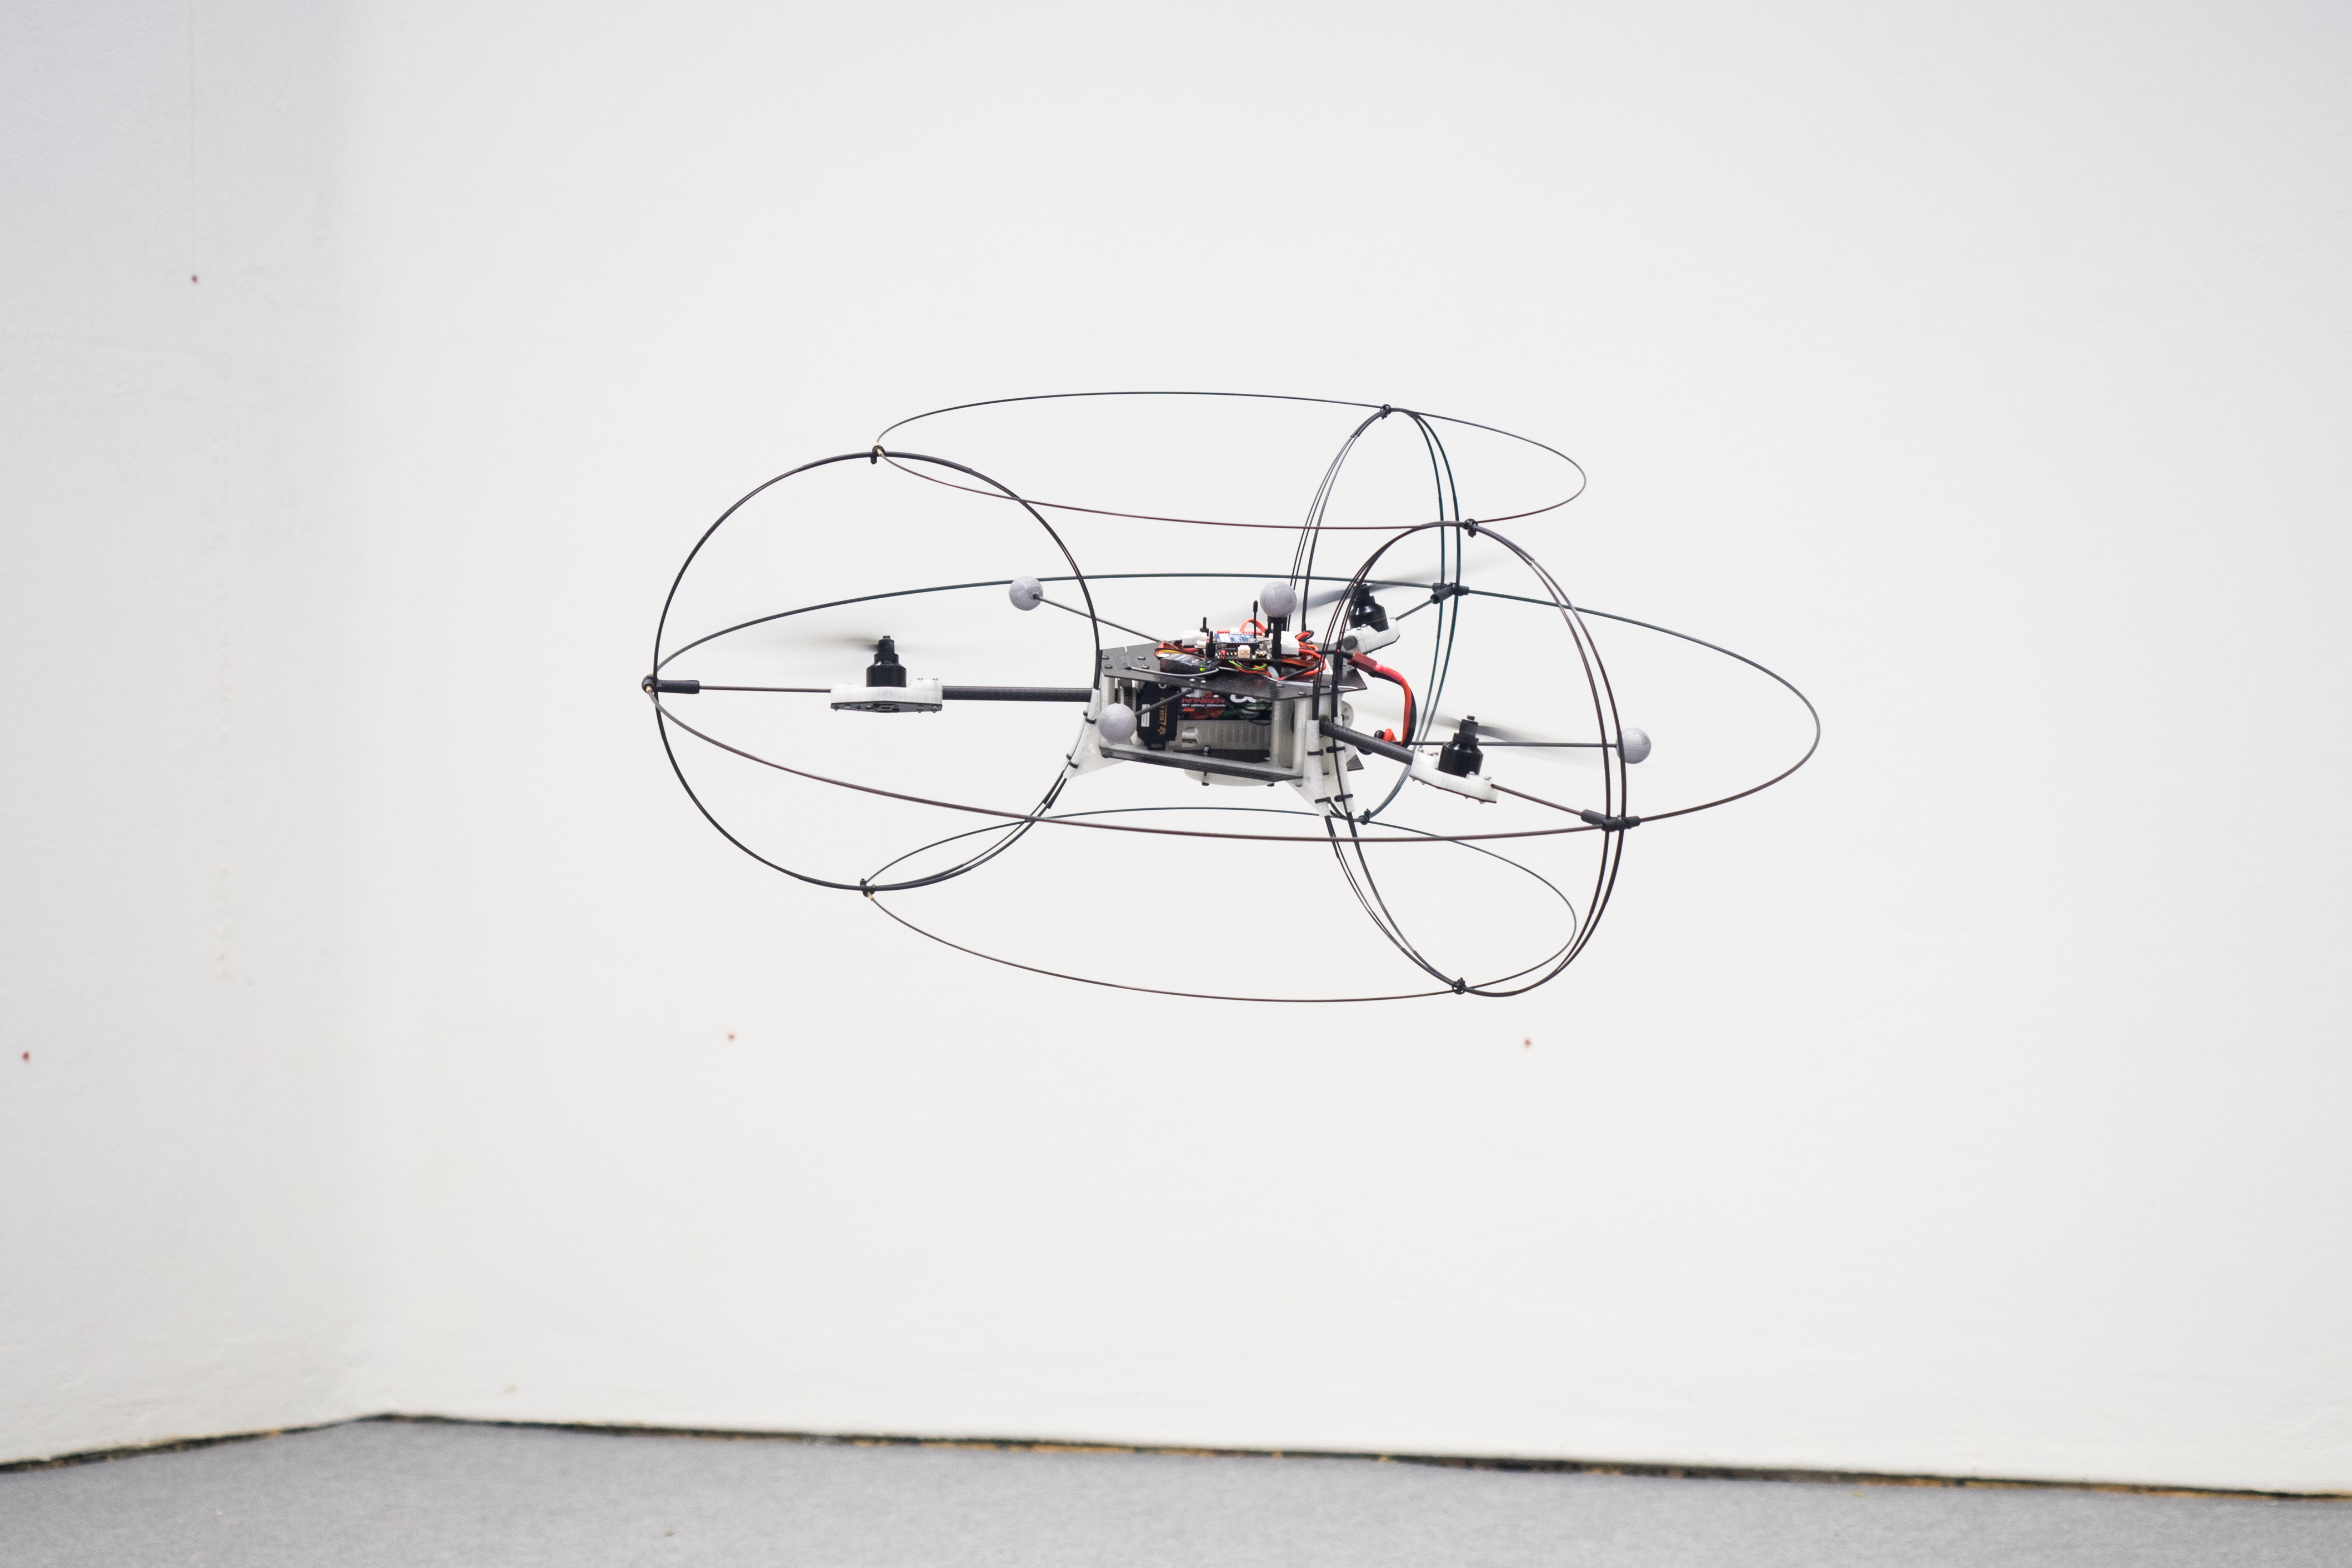
\includegraphics[width=.45\linewidth]{TriV4.jpg}
 \caption{LSR-Quad- and Tricopter}
 \label{fig:LSRQuadAndTri}
\end{figure}

The developed tricopter shown in \autoref{fig:LSRQuadAndTri} is characterized by the three independently tiltable, propeller supporting arms.
The central body and the arms are a sandwich construction of carbon-fiber plates and tubes and 3d-printed parts.
The outer carbon-fiber rings serve as collision protection and landing gear.
The vehicle has an outer diameter of about $0.8\,\unit{m}$ and a mass of about $1.2\,\unit{kg}$.

The tilting mechanism is driven by a standard hobby servo motor that is connected to a gear on the arm by a toothed-belt and allows for tilt angles of $\pm 75^\circ$.
The three $10\,\unit{inch}$ propellers are each driven by a brushless dc-motor (BLDC) capable of angular velocities up to $120\,\unit{Hz}$, corresponding to a maximum thrust of $8\,\unit{N}$.
As energy source the tricopter carries a $14.8\,\unit{V}$, $2.2\,\unit{Ah}$ LiPo battery that allows for up to $15\,\unit{min}$ of autonomous flight.

Two types of sensors are used by the tricopter:
An inertial measurement unit (IMU) VN100s from \textsc{VectorNav} is mounted on the central body to measure its angular velocity and acceleration and provide attitude estimates.
An external camera-based motion capture system from \textsc{Vicon} measures position and attitude by way of reflective markers on the tricopter.

A standard two-joystick remote control is used as a reliable and near real-time user interface to the vehicle while a pair of XBee S6B Wi-Fi modules provides a two-way communication link with a groundstation PC.
The important hardware components are summarized in \autoref{fig:MulticopterRealizationOverview}.

The onboard electronics consist mainly of a custom-built mainboard and three identical motor drivers. The mainboard contains an Atmel AT32UC3C 32-bit, 66~\unit{MHz} microcontroller with FPU and is tasked with executing all control algorithms.
Although compact brushless-dc motor drivers are ubiquitous, available products typically lack explicit speed control. 
Moreover, while the rotor speed is implicitly known to the driver through electrical commutation, speed feedback necessary for an external control implementation is usually not provided. 
As a result, a custom module was developed that provides such a measurement while implementing an underlying current controller to drive the motor. 
This solution allows for rapid propeller dynamics described further in (??) that include active braking, achieved by feeding current back into the battery.


\begin{figure}[t]
 \centering
 \footnotesize
 \newcommand{\macGroundstation}{\textcolor{white}{\textbf{Groundstation} (Win7 PC)}}
 \newcommand{\macMulticopterRealization}{\textcolor{white}{\textbf{Multicopter}}}
 \newcommand{\macRBSI}{\textcolor{white}{\textbf{rigid}}}
 \newcommand{\macRBSII}{\textcolor{white}{\textbf{body}}}
 \newcommand{\macRBSIII}{\textcolor{white}{\textbf{system}}}
 \newcommand{\macMCI}{\textcolor{white}{\textbf{main}}}
 \newcommand{\macMCII}{\textcolor{white}{\textbf{controller}}}
 \input{graphics/MulticopterRealizationOverview.pdf_tex}
 \caption{Multicopter Hardware realization}
 \label{fig:MulticopterRealizationOverview}
%\end{figure}
\vspace{5mm}
 \input{graphics/MicocontrollerCodeStructure.pdf_tex}
 \caption{Controller code structure}
 \label{fig:MicocontrollerCodeStructure}
%\begin{figure}[hb]
% \vspace{5mm}
%  \footnotesize
%  \input{graphics/StructureMulticopterAgent.pdf_tex}
%  \caption{Structure of the Multicopter Agent}
%  \label{fig:StructureMulticopterAgent}
\end{figure}